\documentclass[tikz,border=4pt]{standalone}
\usepackage{ctex}
\usepackage{amsmath}
\usepackage{pgfplots}
\pgfplotsset{compat=1.18}

% p9-01a: 反比例函数 k>0（y=6/x），图象在第一、三象限
\begin{document}
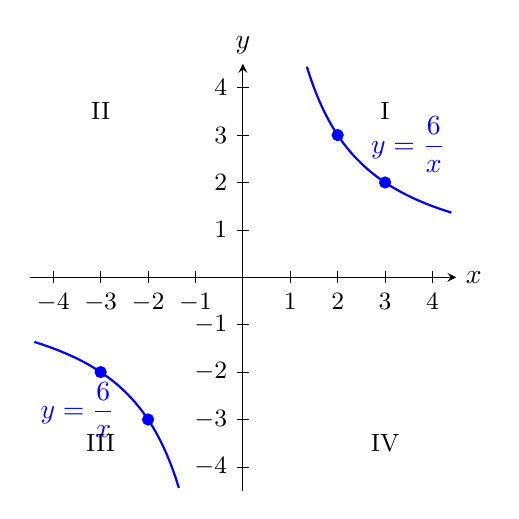
\begin{tikzpicture}
\begin{axis}[
  width=7cm, height=7cm,
  axis lines=center,
  xlabel={$x$}, ylabel={$y$},
  every axis x label/.style={at={(axis cs:4.5,0)}, anchor=west},
  every axis y label/.style={at={(axis cs:0,4.5)}, anchor=south},
  xmin=-4.5, xmax=4.5,
  ymin=-4.5, ymax=4.5,
  xtick={-4,-3,-2,-1,1,2,3,4},
  ytick={-4,-3,-2,-1,1,2,3,4},
  tick style={color=black},
  ticklabel style={font=\small},
  clip=true,
]
  % y = 6/x, 第一象限
  \addplot[blue, thick, domain=1.35:4.4, samples=80] {6/x};
  % y = 6/x, 第三象限
  \addplot[blue, thick, domain=-4.4:-1.35, samples=80] {6/x};

  % 标记几个点
  \addplot[blue, only marks, mark=*, mark size=2pt] coordinates {(1,6) (2,3) (3,2) (6,1)};
  \addplot[blue, only marks, mark=*, mark size=2pt] coordinates {(-1,-6) (-2,-3) (-3,-2) (-6,-1)};

  % 函数标签
  \node[right, blue] at (axis cs:2.5, 2.8) {$y=\dfrac{6}{x}$};
  \node[left, blue] at (axis cs:-2.5, -2.8) {$y=\dfrac{6}{x}$};

  % 象限标注
  \node[font=\small] at (axis cs:3,3.5) {I};
  \node[font=\small] at (axis cs:-3,3.5) {II};
  \node[font=\small] at (axis cs:-3,-3.5) {III};
  \node[font=\small] at (axis cs:3,-3.5) {IV};
\end{axis}
\end{tikzpicture}
\end{document}
